\documentclass[smallextended]{svjour3}
%\documentclass[11point]{article}

% definitions used by included articles, reproduced here for 
% educational benefit, and to minimize alterations needed to be made
% in developing this sample file.
\usepackage{color,epsfig,amssymb,amsmath,subfigure,url}

%%%%%%%%%%%%   Macros defined by Gelb %%%%%%%%%%%%%%%%
\newcommand{\vf}{\boldsymbol f}

\newcommand{\mF}{\mathsf F}
\newcommand{\mP}{\mathsf P}
\newcommand{\mPhi}{\mathsf \Phi}

\newcommand{\hf}{\hat{f}}
\newcommand{\hvf}{\hat{\vf}}

\newcommand{\spB}{\mathcal B}

\newcommand{\se}{{\rm e}}

\newcommand{\bZ}{{\mathbb Z}}

%%%%%%%%%%%%%%%%%%%%%%%%%%%%%%%%%%%%%%%%%%%%%

\topmargin-0.5in
\textheight9in
\oddsidemargin0in
\evensidemargin0in
\textwidth6.6in

\title{Awesome Title}

\author{Ben Adcock\thanks{Department of Mathematics, Simon Fraser University, Burnaby, BC V5A 1S6 ({\tt ben\_adcock@sfu.ca})}  \and
	Rick Archibald\thanks{Computer Science and Mathematics Division, Oak Ridge National Laboratory, Oak Ridge, TN 37831 ({\tt archibaldrk@ornl.gov})}  \and
        Anne Gelb\thanks{School of Mathematical and Statistical Sciences, Arizona State University, Tempe, AZ, 85287 ({\tt annegelb@asu.edu})}\and
        Guohui Song\thanks{Department of Mathematics, Clarkson University, Potsdam, NY 13699. ({\tt gsong@clarkson.edu})} \and 
        Rodrigo B. Platte\thanks{School of Mathematical and Statistical Sciences, Arizona State University, Tempe, AZ, 85287 ({\tt rbp@asu.edu})} \and
        Edward G. Walsh \thanks{Department of Neuroscience, Brown University, Providence, RI 02912 ({\tt edward\_walsh@brown.edu})}}

\graphicspath{{./pictures/}}

\begin{document}

\newtheorem{thm4}{Theorem}
\newtheorem{thm5}{Theorem}
\newtheorem{thm}{Theorem}
%\newtheorem{remark}{Remark}
\newtheorem{defn}[thm5]{Definition}
%\newtheorem{example}[thm4]{Example}
%\newtheorem{algorithm}[thm]{Algorithm}
\newtheorem{algorithm}{Algorithm}

\maketitle
\begin{abstract}

\end{abstract}


\keywords{Fourier Data \and  $l^1$ regularization \and Split Bregman \and MRI}

\section{Introduction}
\label{sec:introduction}

\section{Methods}
\label{sec:methods}
\subsection{Measurements}

\begin{equation}
\label{eq:2Dhatf}
S(k_x,k_y,t) =  \iint\limits_{\Omega} m(x,y)e^{-R^*(x,y)t+if(x,y)t}e^{-ik_xx-ik_yy}\partial\Omega 
\end{equation}
\subsection{Sampling}
\subsection{Fourier Frames}
\subsection{TV optimization}
\section{Numerical}
\label{sec:numerical}


\begin{figure}[h!]
\centering
\subfigure[$Interpolation Error$]{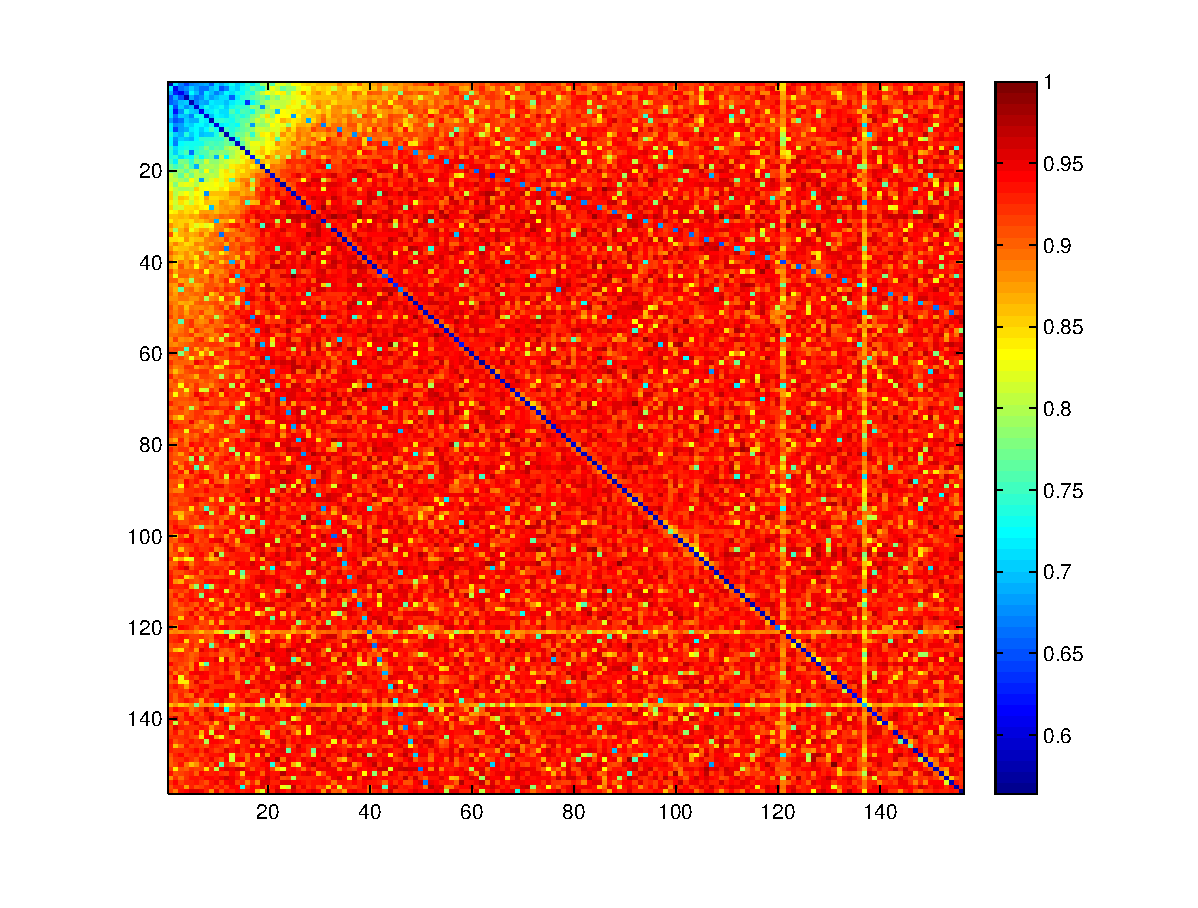
\includegraphics[width=.24\textwidth]{normalized_err}}
\subfigure[$Unique Sample Points$]{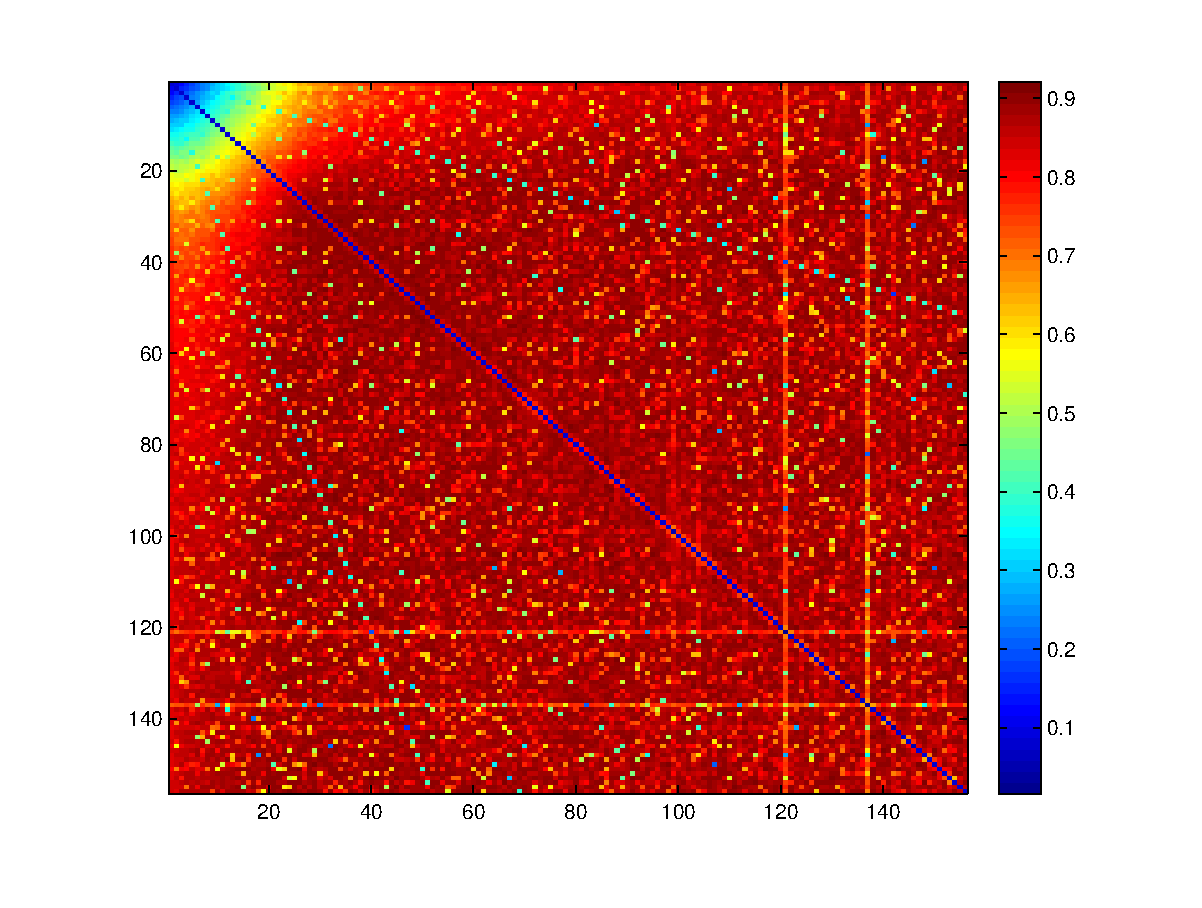
\includegraphics[width=.24\textwidth]{normalized_unique}}

\caption{(a) Interpolation Error and  (b) Unique Sample Points are factors in choosing spiral MRI}
\label{fig:sample pattern}
\end{figure}

\begin{figure}[h!]
\centering
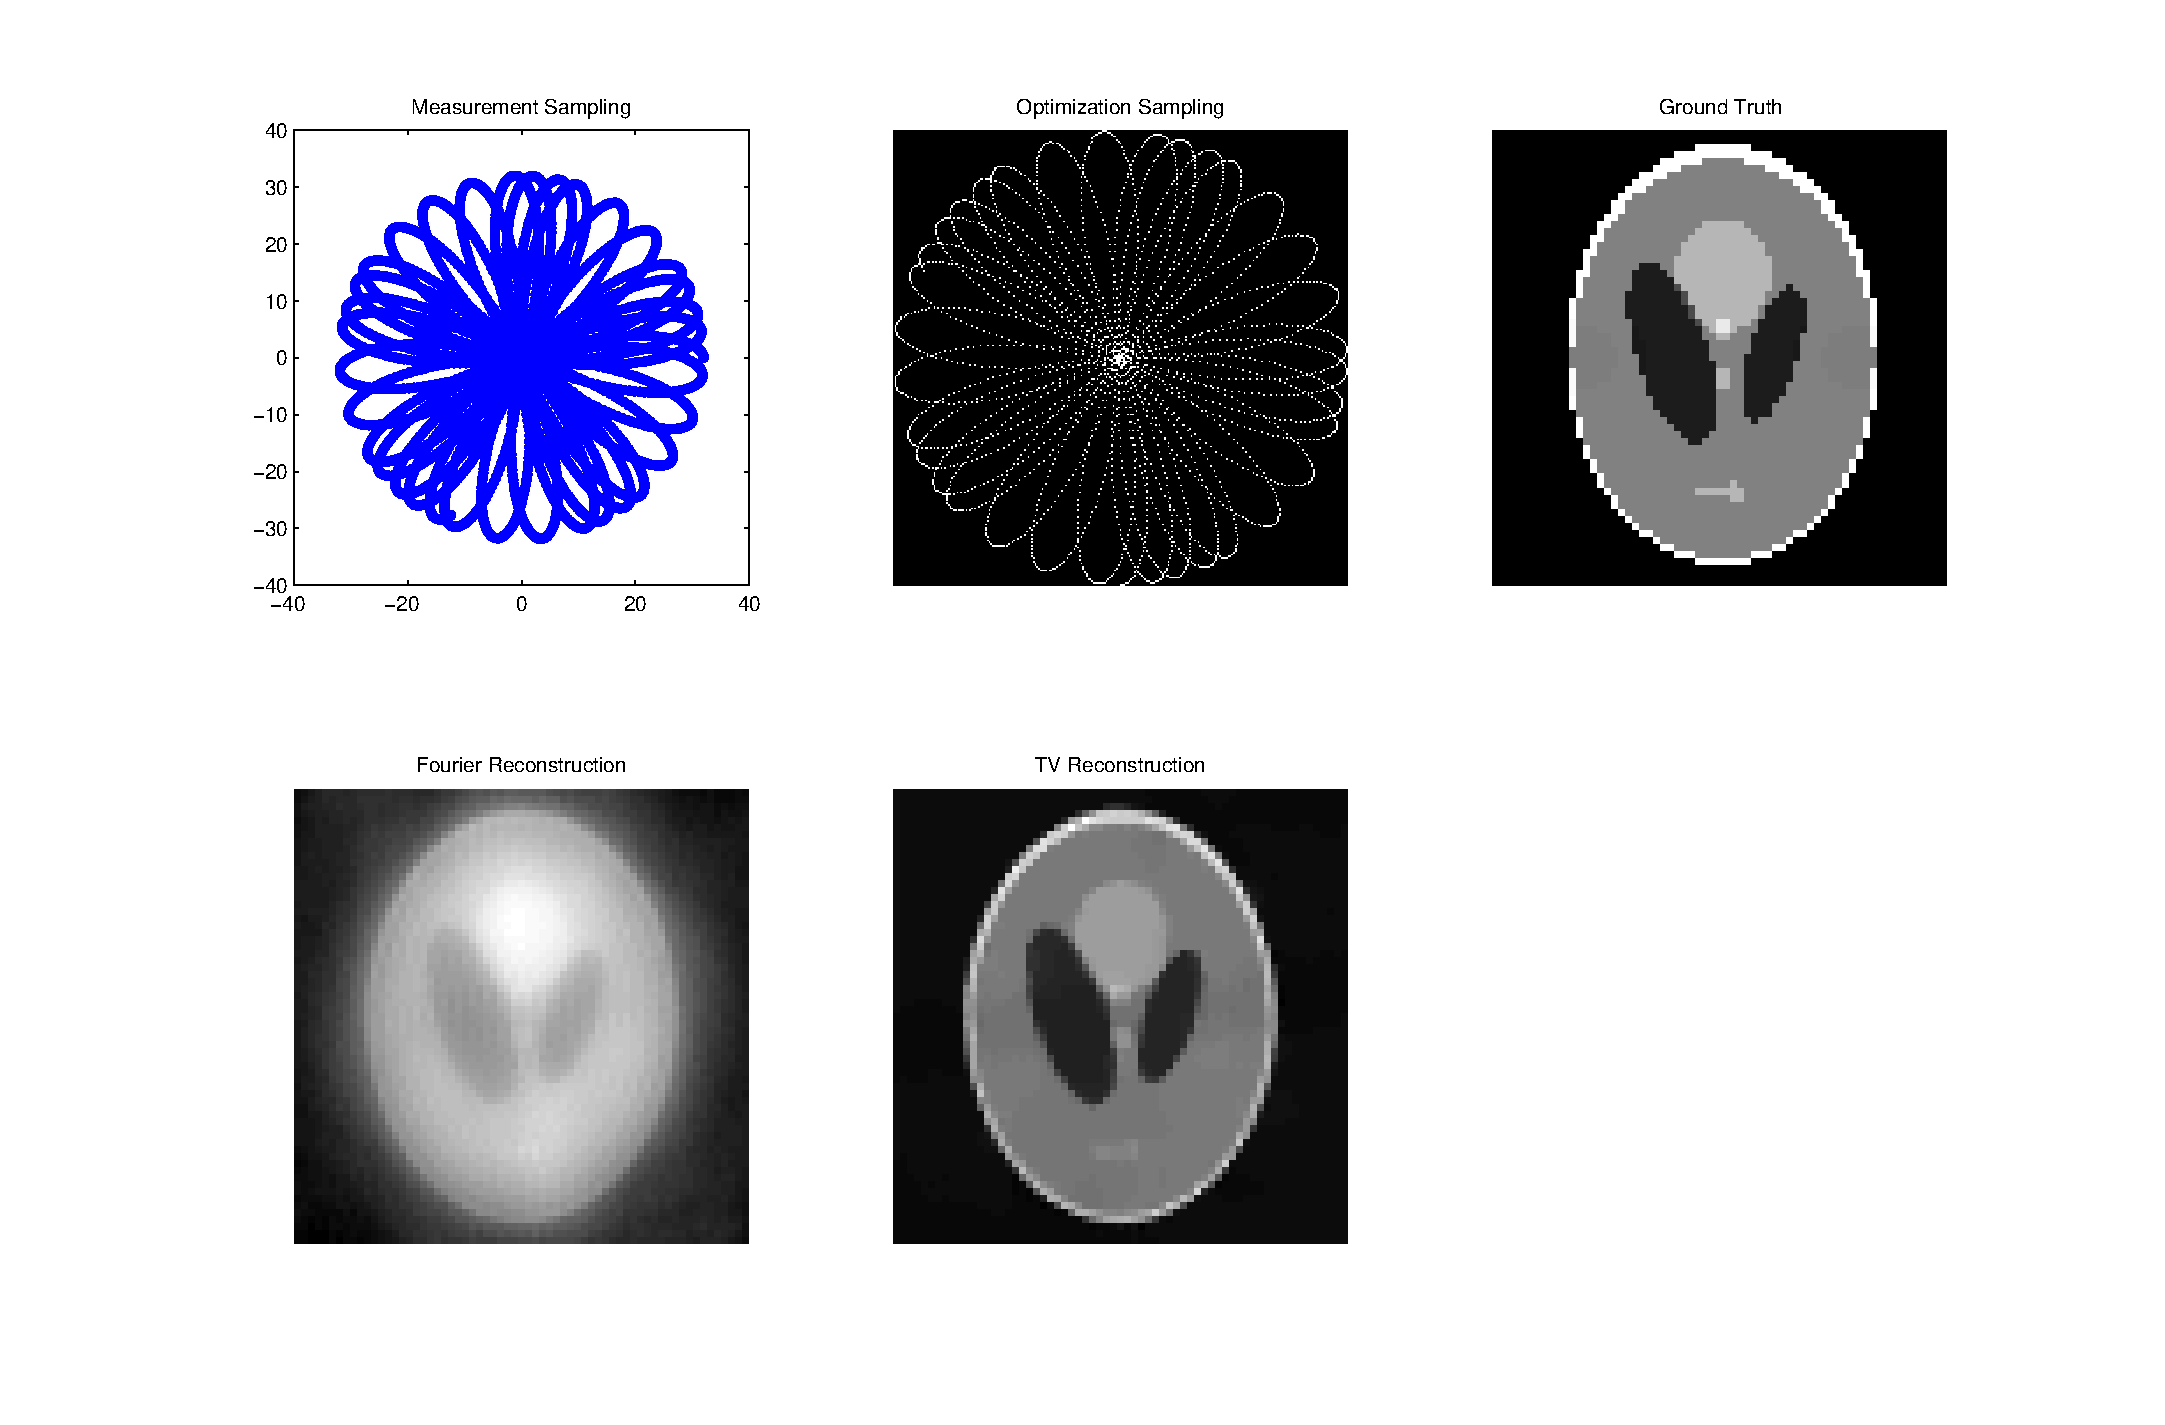
\includegraphics[width=.5\textwidth]{eg1_window_samp}
\caption{Time slice}
\label{fig:sim_eg_timeslice}
\end{figure}

\begin{figure}[h!]
\centering
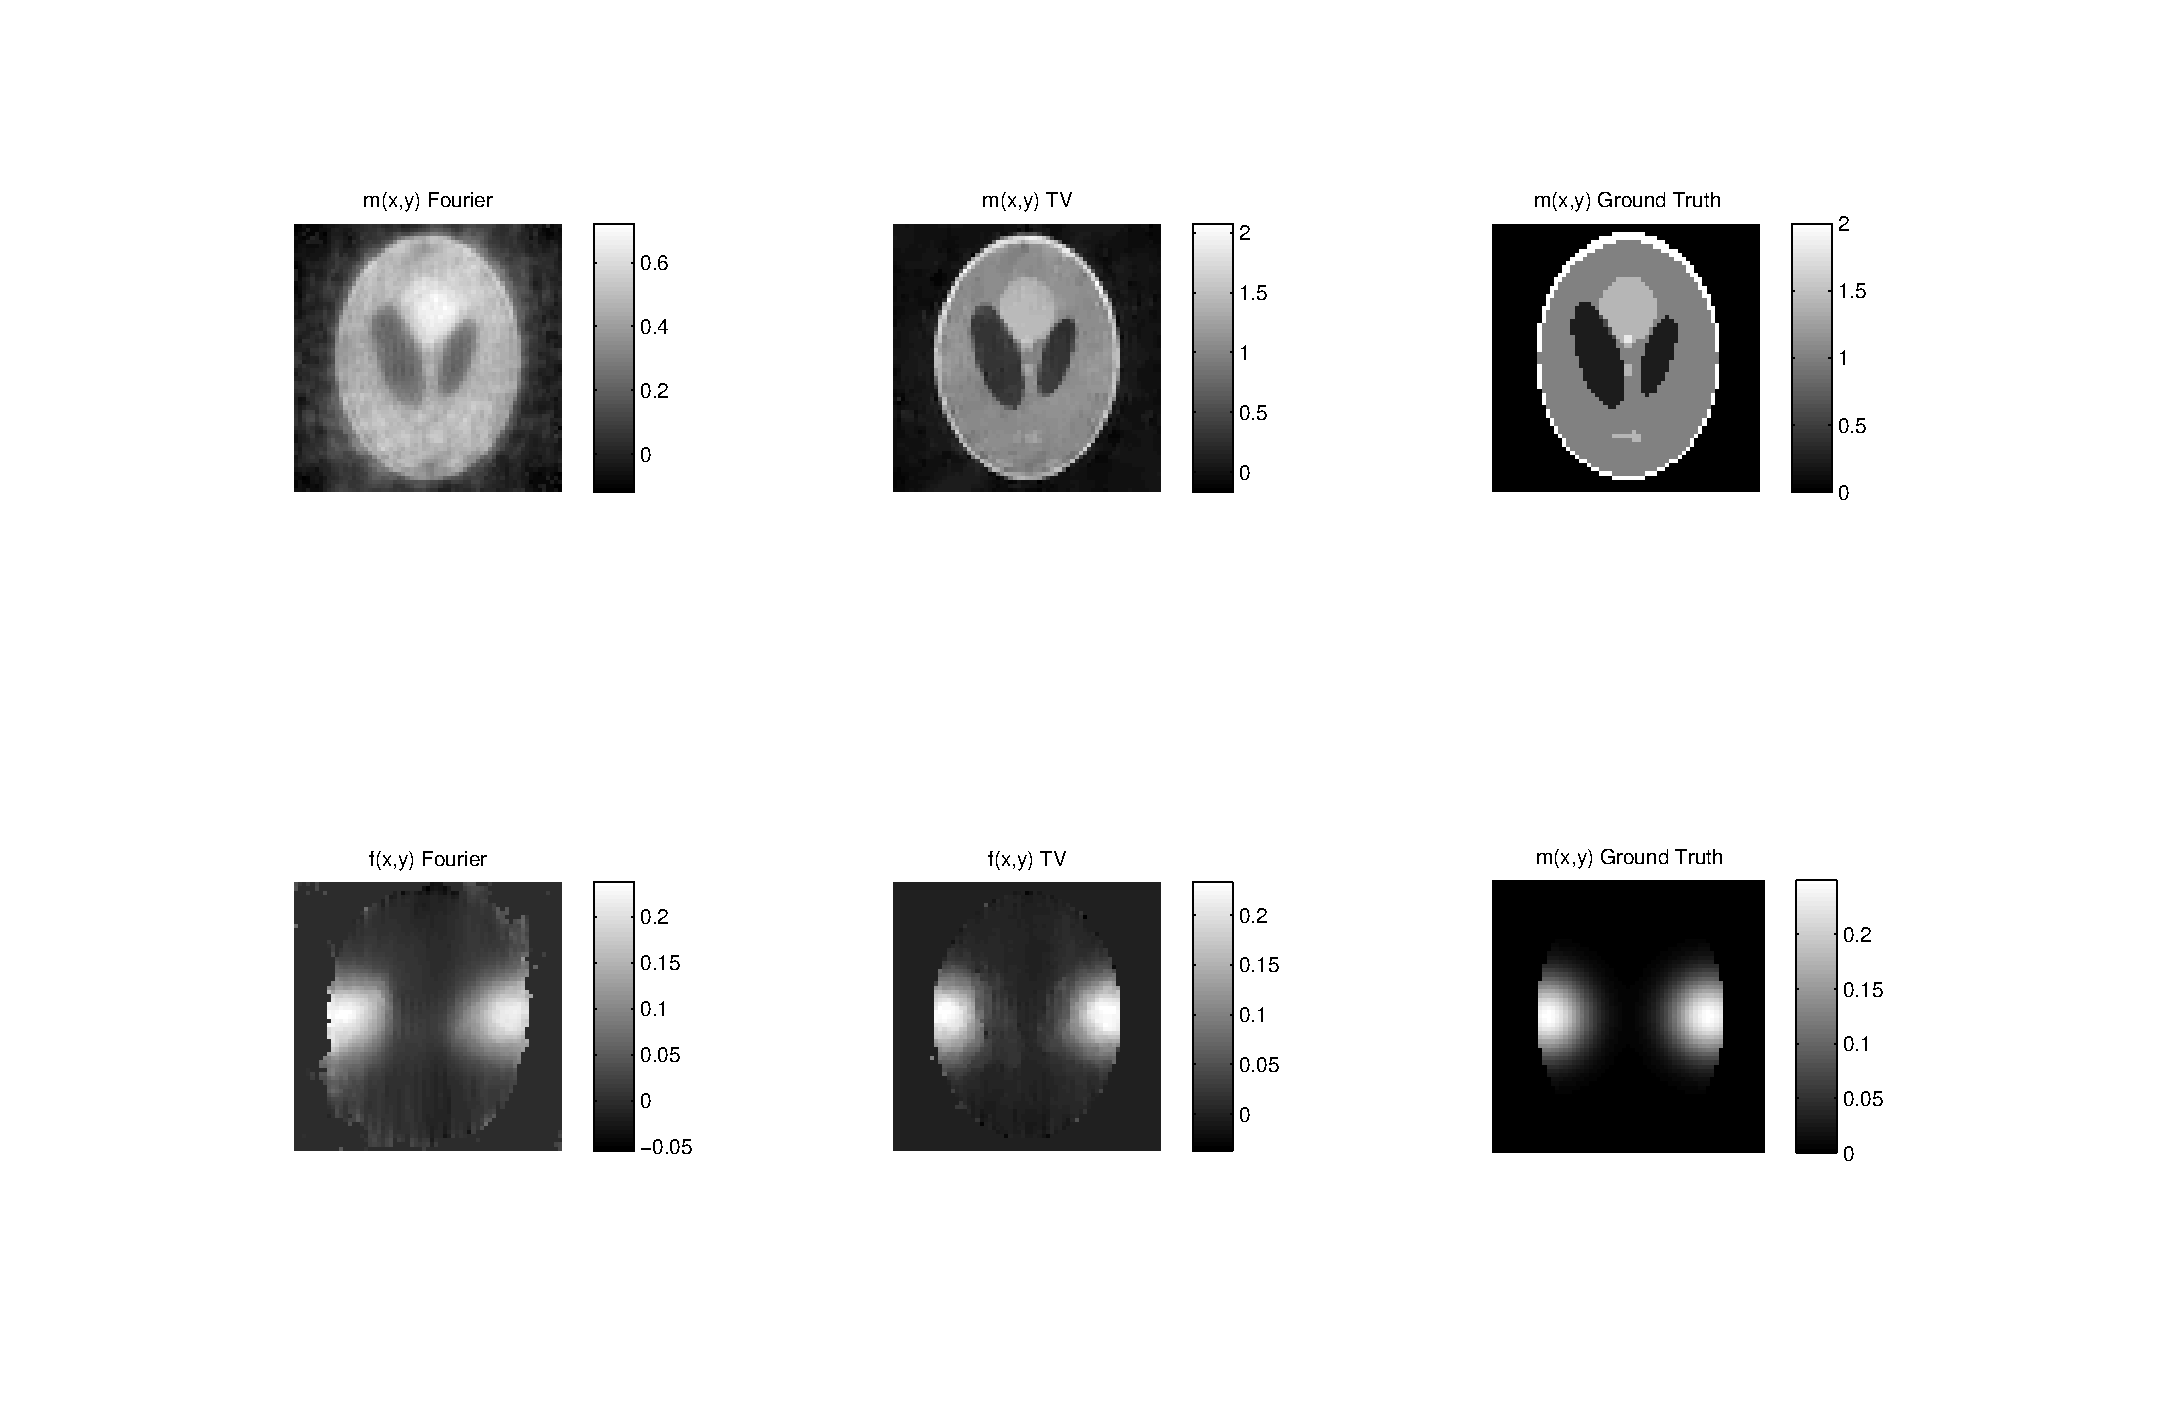
\includegraphics[width=.5\textwidth]{eg1}
\caption{Time series analysis}
\label{fig:sim_eg_timeseries}
\end{figure}
\section{Conclusion}
\label{sec:conclusion}

%\begin{AMS}
%41A25,41A45,41A63.
%\end{AMS}

%\pagestyle{myheadings}
%\thispagestyle{plain}
%\markboth{Archibald, Gelb, $\&$ Platte}{Reconstruction of Partially Sampled Fourier Data}


\subsection*{Acknowledgments}
\label{sect:acks}
This work is supported in part by grants NSF-DMS 1216559 and AFOSR FA9550-12-1-0393.   The submitted manuscript is based upon work, authored in part by contractors [UT-Battelle LLC, manager of Oak Ridge National Laboratory (ORNL)], and supported by the U.S. Department of Energy, Office of Science, Office of Advanced Scientific Computing Research, Applied Mathematics program. Accordingly, the U.S. Government retains a non-exclusive,  royalty-free license to publish or reproduce the published form of this contribution, or allow others to do so, for U.S. Government purposes.

\bibliography{AIMS15}
\bibliographystyle{acm}


\end{document}

